\documentclass[a4paper, 12pt]{article}
\usepackage[utf8]{inputenc}
\usepackage[slovene]{babel}

\usepackage{amsthm}
\usepackage{amsmath, amssymb, amsfonts}
\usepackage{relsize}
\usepackage{graphicx}
\usepackage{etoolbox}
\usepackage{setspace}
\graphicspath{ {./Slike/} }
\usepackage[
top    = 3.cm,
bottom = 3.cm,
left   = 3.cm,
right  = 3.cm]{geometry}
\usepackage{hyperref}
\usepackage{mathtools}
\usepackage{authblk}
\usepackage{makecell}
\usepackage[nottoc]{tocbibind}
\usepackage{algorithm}
\usepackage[noend]{algpseudocode}

\makeatletter
\def\BState{\State\hskip-\ALG@thistlm}
\makeatother


\newtheorem{definicija}{Definicija}
\newtheorem{posledica}{Posledica}

\begin{document}

\begin{titlepage}
    \begin{center}
        \textsc{\LARGE Univerza v Ljubljani}\\[0.5cm]
        {\Large Fakulteta za matematiko in fiziko}\\[3cm]
        {\large Finančni praktikum}\\[0.5cm]
        {\huge Največje neodvisne množice z lokalnim iskanjem}\\[10.0cm]
    \end{center}

    \begin{minipage}{0.4\textwidth}
		\begin{flushleft}
			\large
			\textit{Avtorja:}\\
			Jaka Mrak \\
			Žiga Gartner 
		\end{flushleft}
	\end{minipage}
	~
	\begin{minipage}{0.4\textwidth}
		\begin{flushright}
			\large
			\textit{Mentorja:}\\
			prof. dr. Sergio \textsc{Cabello} \\
			doc. dr. Janoš \textsc{Vidali}
		\end{flushright}
	\end{minipage}
	
	\vfill\vfill\vfill 
	\begin{center}
	{\large{Ljubljana, \today}} 
    \end{center}
	\vfill 

\end{titlepage}

\tableofcontents

\newpage

\section{Navodilo}

Naloga je iskanje največje neodvisne množice v grafu $G = (V,E)$ s pomočjo celoštevilskega linearnega programiranja. Velike neodvisne množice v grafu lahko poiščemo s pomočjo metode lokalnega iskanja.
Začnemo s poljubno neodvisno množico $U  \subseteq V$, kjer $k$ vozlišč nadomestimo s $k + 1$ vozlišči tako, da ohranjamo neodvisnost množice $U$. Konstanta $k$ je dana na začetku. Primerjali bomo metodi
lokalnega iskanja in optimalne rešitve ter primerjali njune rešitve za nekatere preproste grafe.

\section{Opis problema}
\begin{definicija}
    Naj bo $G = (V,E)$ graf. \textbf{Neodvisna množica} $U$, v grafu $G$, je taka podmnožica množice vozlišč $V$, kjer poljubni dve vozlišči iz množice $U$ nista sosednji.
    \textbf{Maksimalna neodvisna množica} v grafu $G$ pa je taka neodvisna množica, kjer ne obstaja vozlišče $v \in V$ in $v \notin U$, ki bi ga lahko dodali množici $U$ in pri tem ohranili neodvisnost množice $U$. Torej
    je neodvisna množica $U$ največja taka, če velja ena od naslednjih dveh lastnosti:
    \begin{enumerate}
        \item $v \in U$
        \item $S(v) \cap U \neq \emptyset,$ kjer je $S(v)$ množica sosedov $v$.
    \end{enumerate}
    \textbf{Največja neodvisna množica} je neodvisna množica, največje možne velikosti, za dan graf $G$. Velikosti največje neodvisne množice, za graf $G$, pa pravimo \textbf{neodvisnostno število} in 
    pogosto označimo $\alpha(G)$.
\end{definicija}

\begin{definicija}
    Celoštevilski linearni program v standardni obliki je dan z matriko $A \in \mathbb{R}^{m \times n}$, vektorjem $b \in \mathbb{R}^{m}$ in vektorjem $c \in \mathbb{R}^{n}$. Iščemo
    $$max<c,x>,$$
    da bodo zadoščeni pogoji
    $$ Ax \leq b, x \geq 0,$$
    kjer je $x \in \mathbb{Z}^{n}.$

\end{definicija}

\begin{posledica}
Problem največje neodvisne množice v grafu $G=(V,E)$ lahko s celoštevilskim linearnim programiranjem modeliramo na sledeč način:
$$max \sum_{v \in V} x_{v},$$
da velja:
$$ x_{v} + x_{w} \leq 1 \ za \ \forall vw \in E,$$
$$ x_{v} \in \{0, 1 \}$$
$$ x_{u} = 
    \begin{cases}
    1, \ za \ u \in U \\
    0, \ za \ u \notin U
    \end{cases}, \text{U neodvisna množica v grafu G.}
$$
\end{posledica}

Največjo neodvisno množico v množici vseh neodvisnih podmnožic grafa $G = (V,E)$ bomo iskali s pomočjo celoštevilskega lineranega programiranja in lokalnega iskanja. \textbf{Lokalno iskanje} temelji na
izbiri začetne neodvisne podmnožiče vozlišč $U \subset V$ v kateri $k$ vozlišč zamenjamo s $k + 1$ vozlišči in pri tem ohranjamo neodvisnost množice $U$.

\newpage

\section{Opis dela}
V nadaljevanju bomo največjo oz. maksimalno množico iskali s pomočjo $CLP$, v Sage, in s pomočjo implementiranega algoritma $nakljucni\_MIS(G)$ kasneje izboljšanega z lokalnim
iskanjem. Algoritme bomo izvajali na grafih, generiranih s pomočjo $\text{Erdős-Rényijevega}\ G(n,p)$ modela. Primerjali bomo maksimalne (ali pa največje) neodvisne množice, ki jih algoritmi poiščejo,
časovno zahtevnost algoritmov, kasneje pa še, kako vpliva spreminjanje števila vozlišč in verjetnosti, v modelu, na velikost maksimalne (ali pa največje) neodvisne množice in 
časovno zahtevnost algoritmov.

\subsection{Generiranje podatkov}
Kot omenjeno, bomo grafe generirali s pomočjo $\text{Erdős-Rényijevega}\ G(n,p)$ modela.

\begin{definicija}
    $\text{Erdős-Rényijev}$ model $G(n, p)$ generira graf z $n$ naključno povezanimi vozlišči. Vsaka povezava je v graf vključena neodvisno, z verjetnostjo $p$.
\end{definicija}

Generirali bomo grafe s konstantima $(n,p)$, z naraščajočim $n$ in konstantnim $p$ ter s konstantim $n$ in naraščajočim $p$. Za generacijo podatkov v Pythonu bomo uporabili
knjižnico $NetworkX$, nato pa objekte grafov, s funkcijo $nx.to\_dict\_of\_lists(graf)$, kjer je $nx$ okrajšava za $NetworkX$, pretvorili še v slovarje list, da bomo lahko grafe uporabljali še v okolju $Sage$.
Grafe, na katerih bomo izvajali algoritme, bomo shranili še v $JSON$ datoteke.


\subsection{Algoritmi}

Za iskanje maksimalne neodvisne množice smo implementirali algoritem $nakljucni\_MIS(G)$, čigar rešitev bomo poizkušali izboljšati še z algoritmom $lokalno\_iskanje(G, I)$. Oba
algoritma bosta kot argument sprejela graf $G$, algoritem $lokalno\_iskanje(G, I)$ pa še neko maksimalno neodvisno množico $I$, grafa $G$.

\begin{algorithm}
\caption{$nakljucni\_MIS(G)$}\label{euclid}
\begin{algorithmic}[1]
\State $\textit{I} \gets \emptyset$
\State $\forall v \in V\ \text{dobi vrednost}\ \textit{P}(v) \in \textit{permutacija}(V)$
\If {$\textit{P}(v) < \textit{P}(w)\ \textit{za}\ \forall w \in \textit{sosedi}(v) $}
\State $ I \gets I \cup v $
\EndIf
\State $V' \gets V \setminus (I \cup \textit{sosedi}(I))$.
\State $E' \gets E \setminus \textit{povezave}(I)$.
\State $\text{return}\  I \cup \textit{MIS}(G'=(V', E'))$
\end{algorithmic}
\end{algorithm}

\begin{algorithm}
    \caption{$lokalno\_iskanje(G, I)$}\label{euclid}
    \begin{algorithmic}[1]
    \State $\textit{I} \gets \emptyset$
    \State $\forall v \in V\ \text{dobi vrednost}\ \textit{P}(v) \in \textit{permutacija}(V)$
    \If {$\textit{P}(v) < \textit{P}(w)\ \textit{za}\ \forall w \in \textit{sosedi}(v) $}
    \State $ I \gets I \cup v $
    \EndIf
    \State $V' \gets V \setminus (I \cup \textit{sosedi}(I))$.
    \State $E' \gets E \setminus \textit{povezave}(I)$.
    \State $\text{return}\  I \cup \textit{MIS}(G'=(V', E'))$
    \end{algorithmic}
    \end{algorithm}

\subsection{Analiza rezultatov}

\begin{figure}[h!]
	\begin{center}
		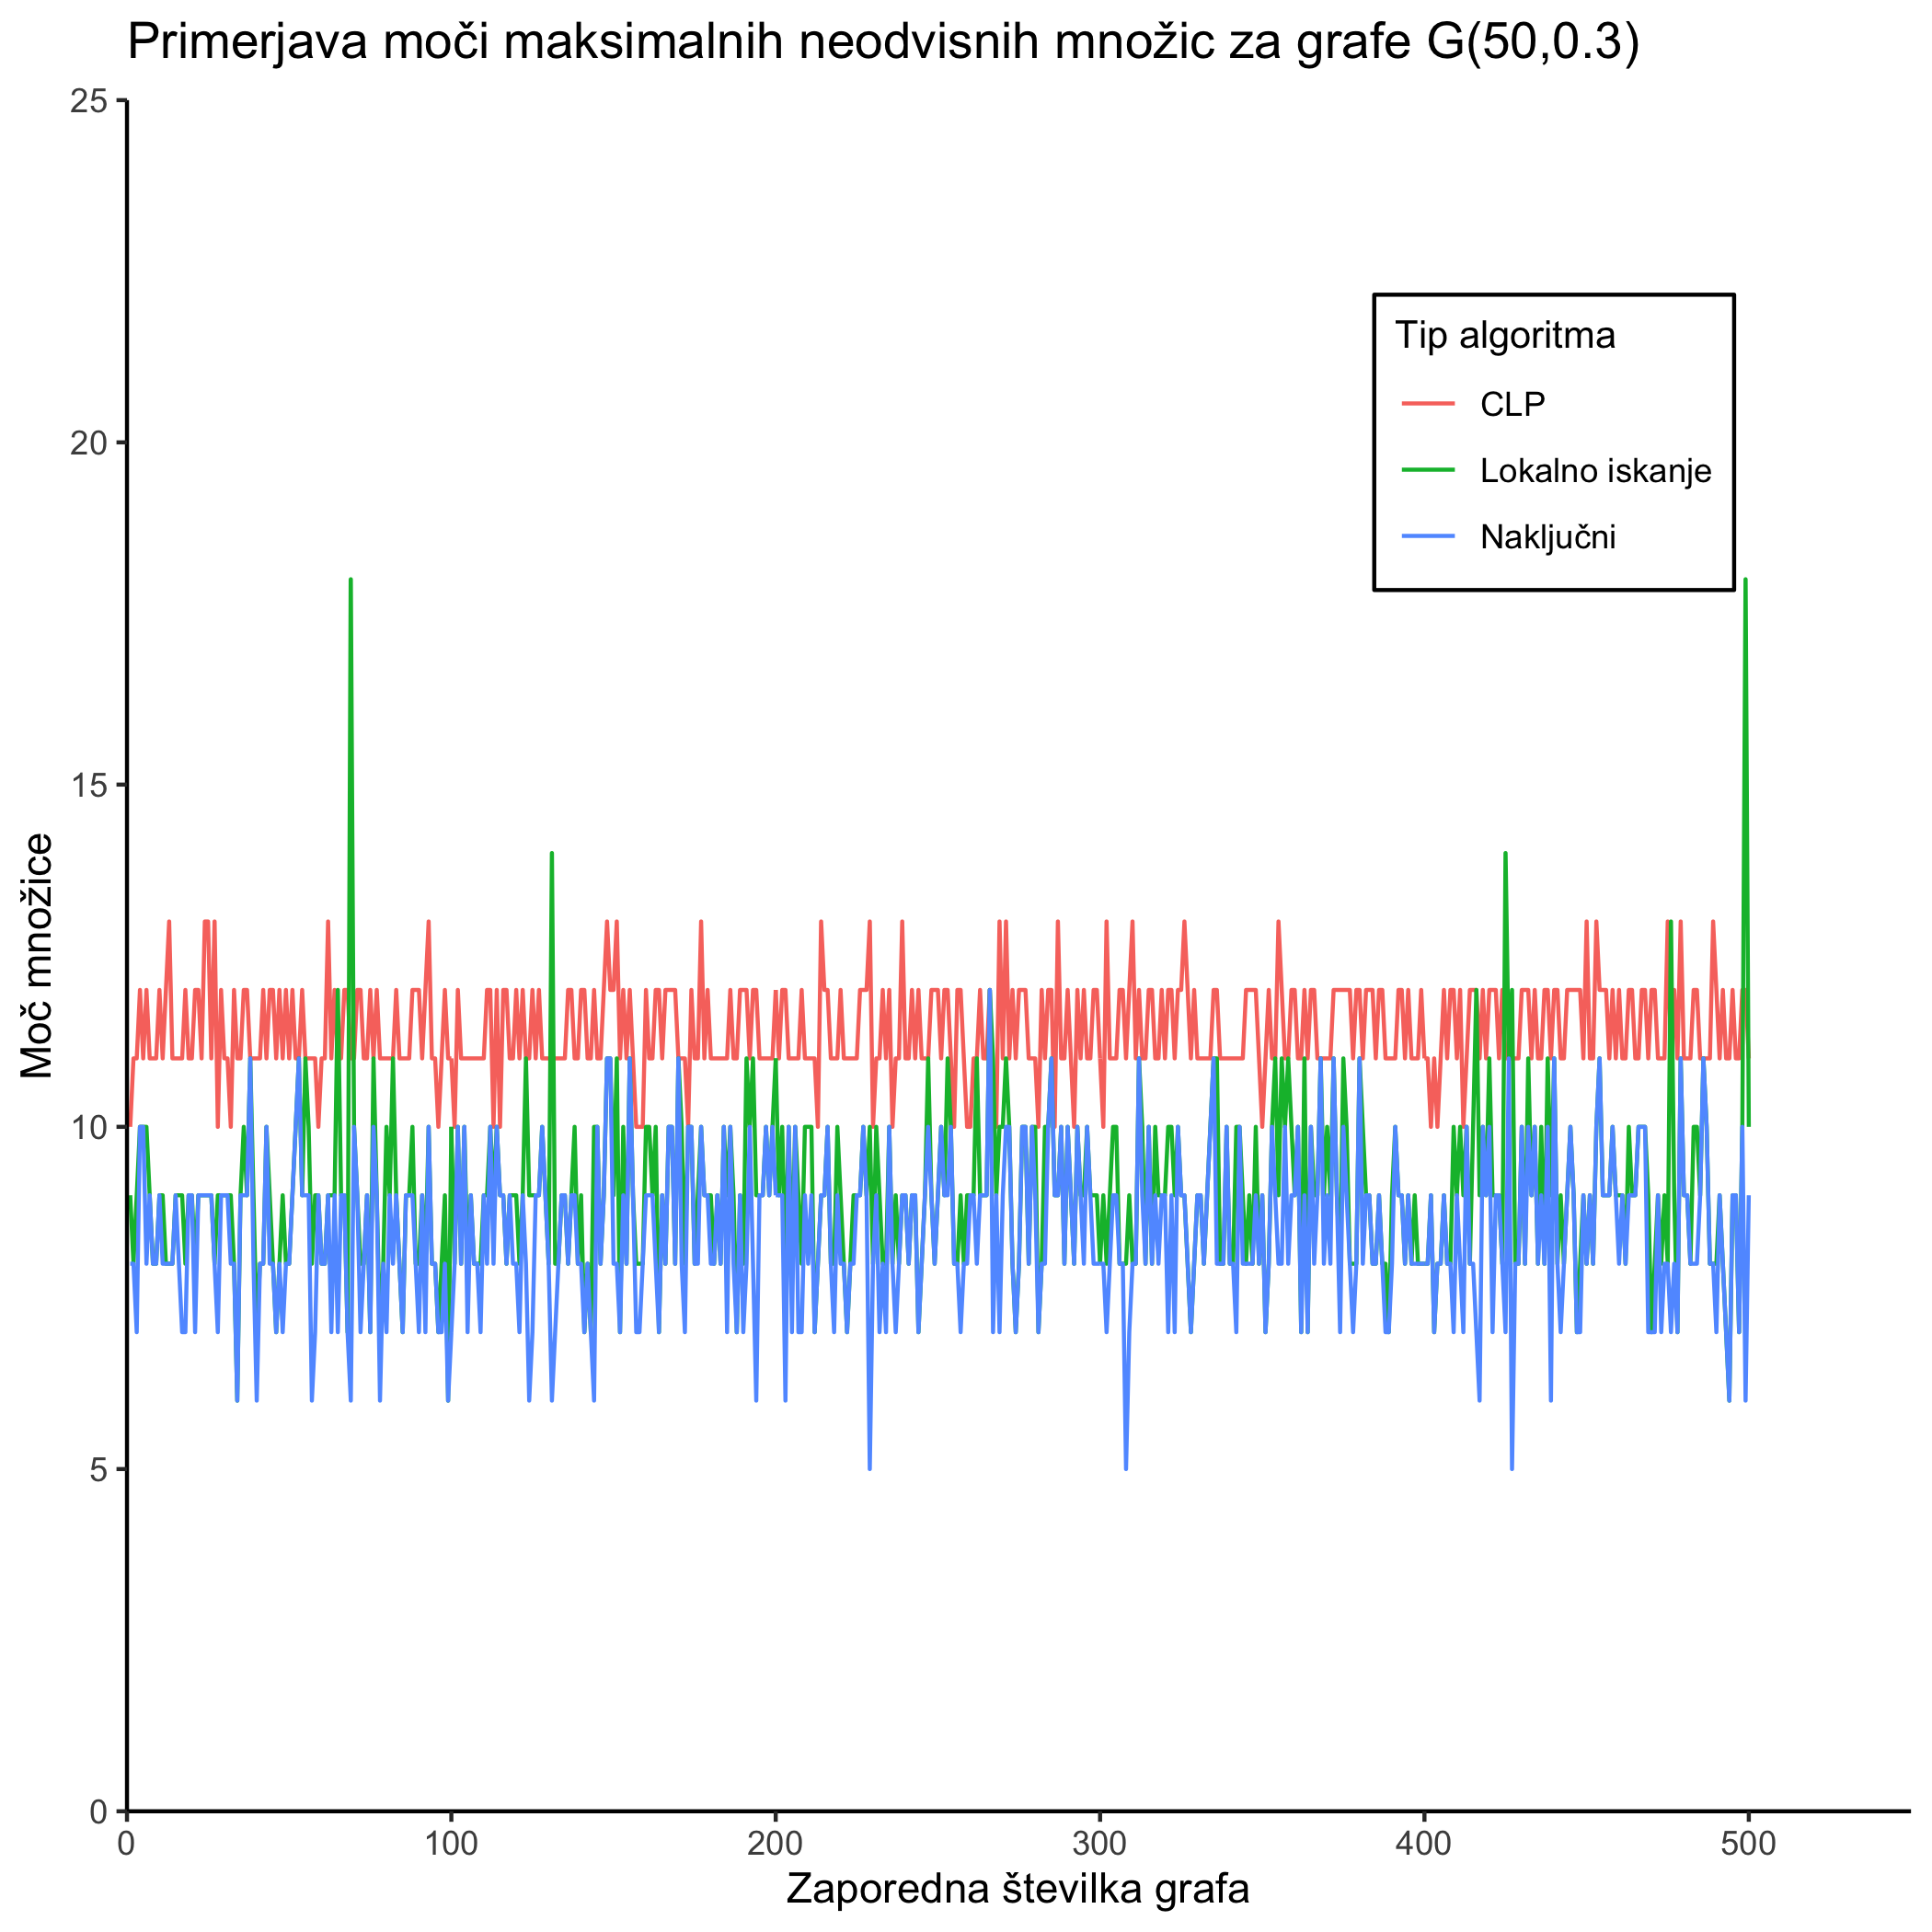
\includegraphics[width=\textwidth]{R_koda/pon-moc.png}
		\caption{Časovnica SPACa.}
	\end{center}
\end{figure}
\vspace{0.5cm}
\begin{figure}[h!]
	\begin{center}
		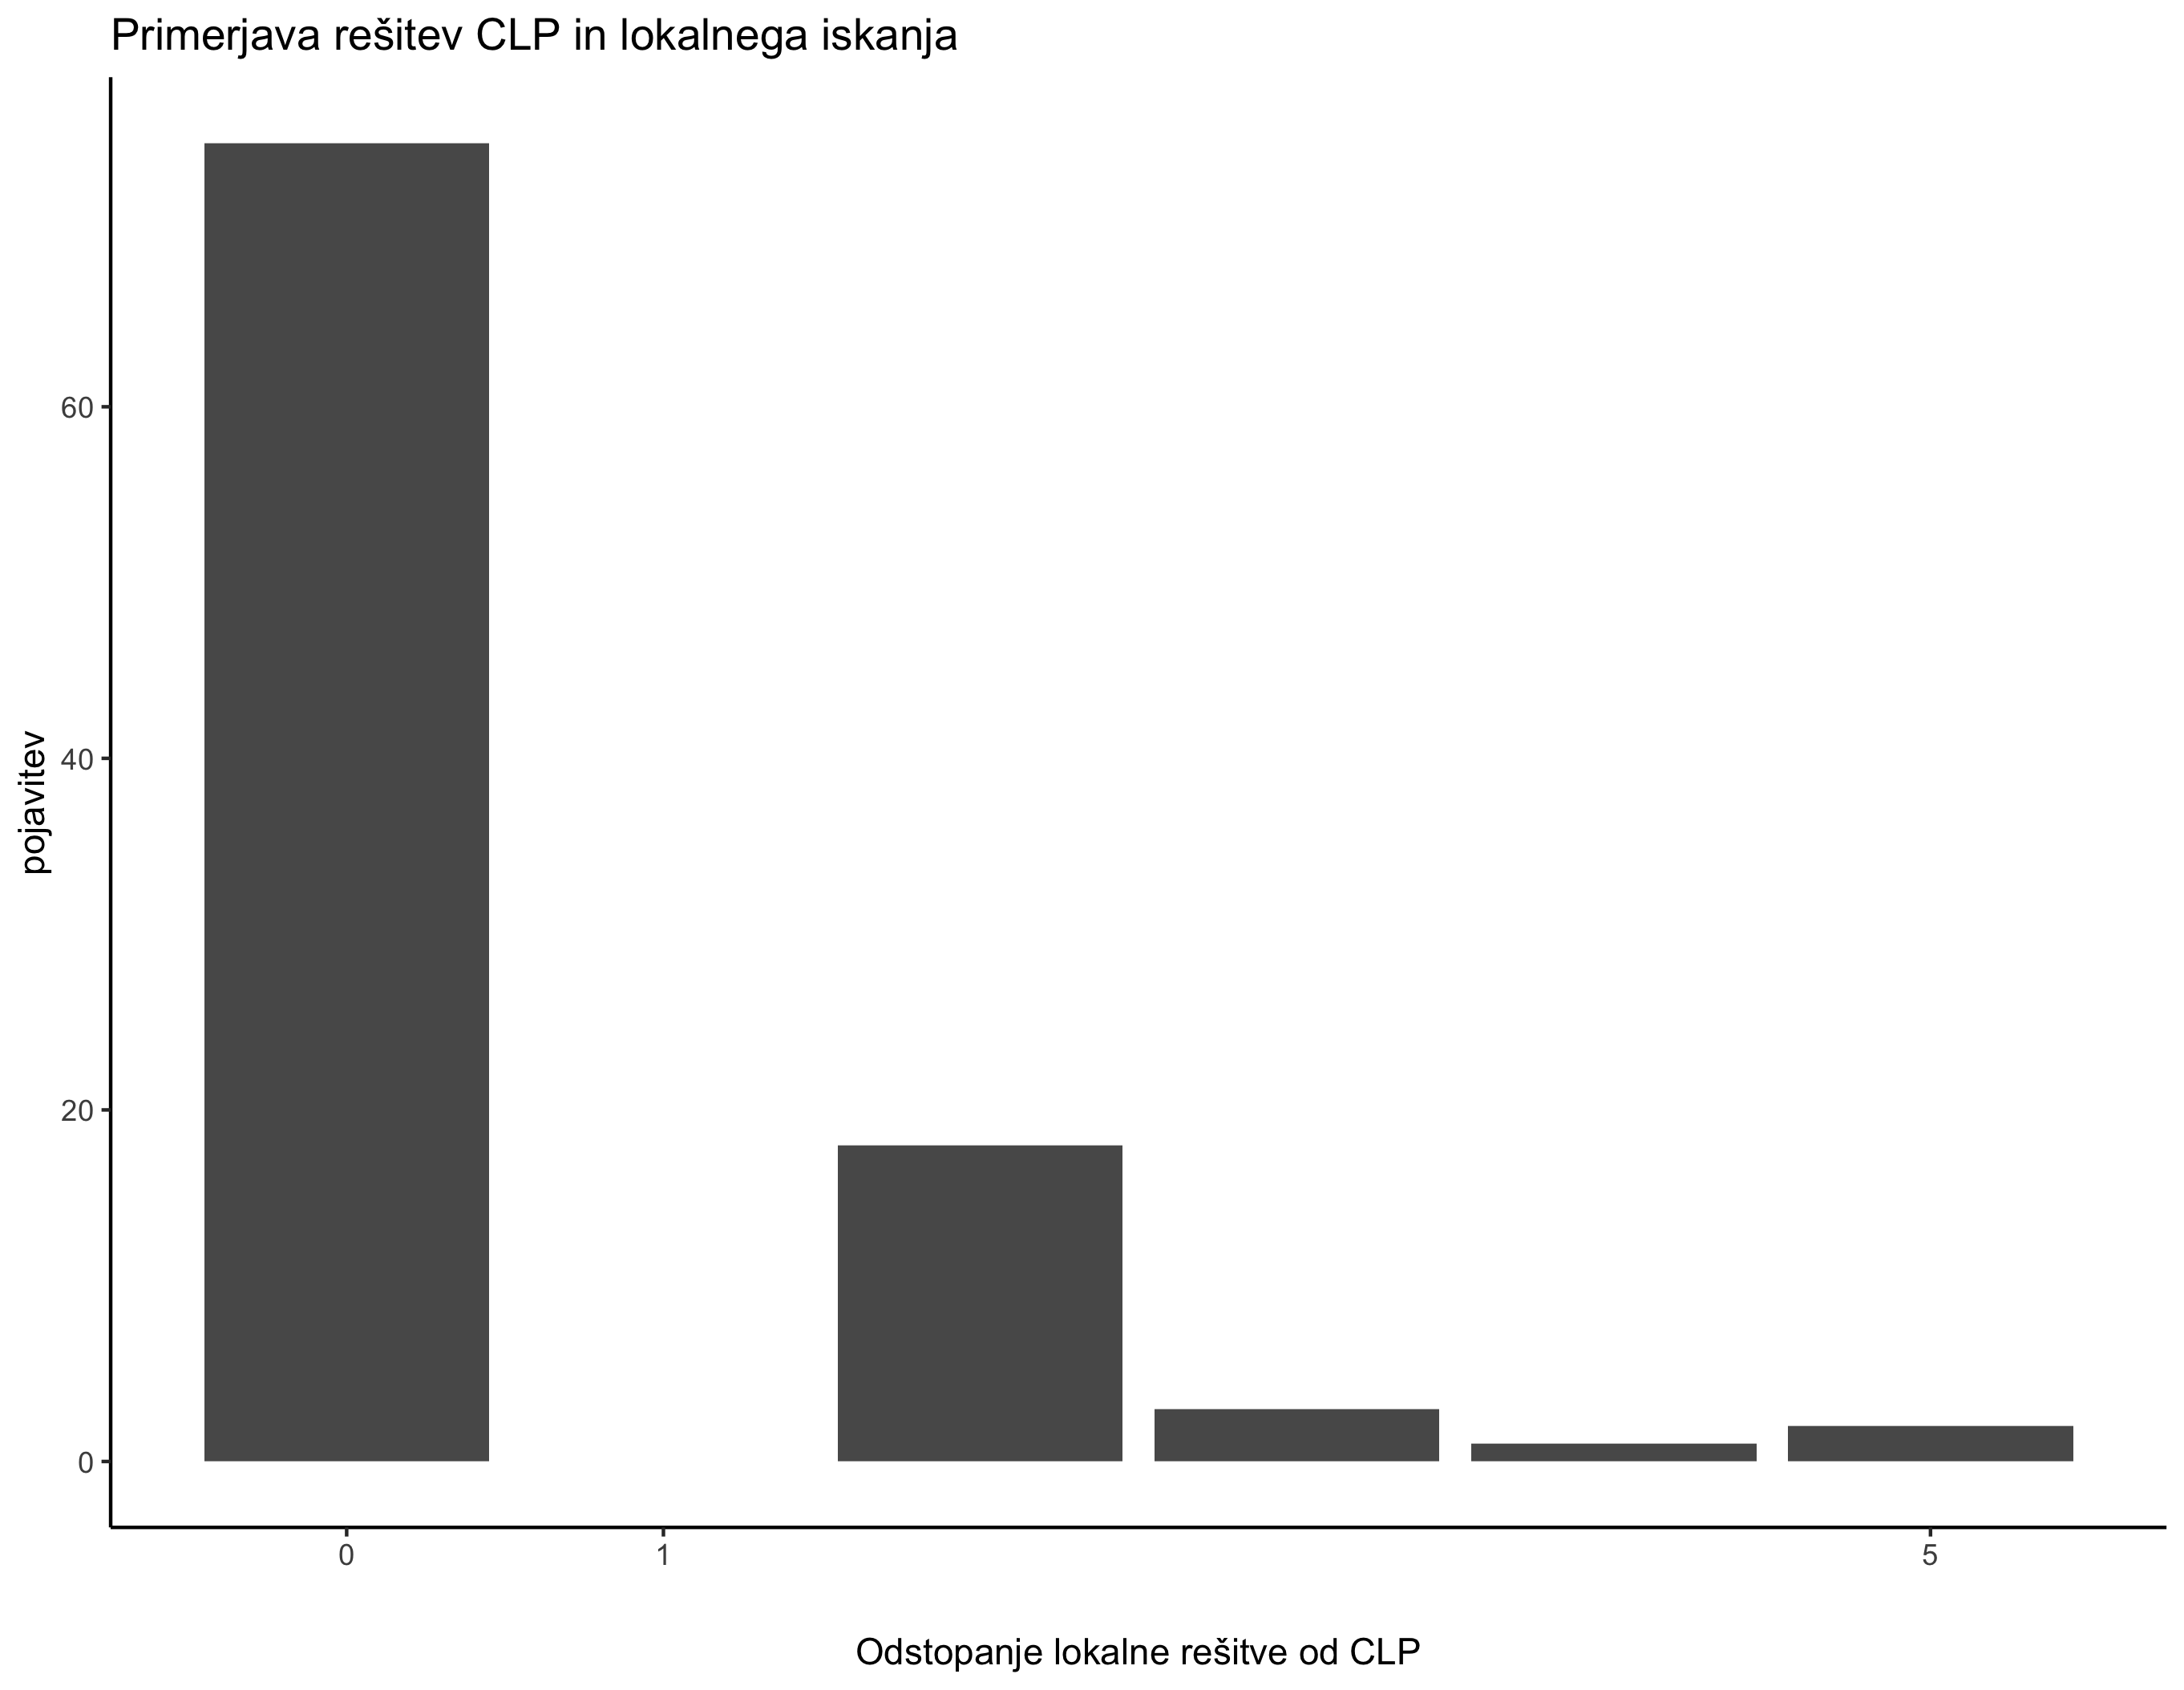
\includegraphics[width=\textwidth]{R_koda/pon-napake.png}
		\caption{Časovnica SPACa.}
	\end{center}
\end{figure}
\vspace{0.5cm}
\begin{figure}[h!]
	\begin{center}
		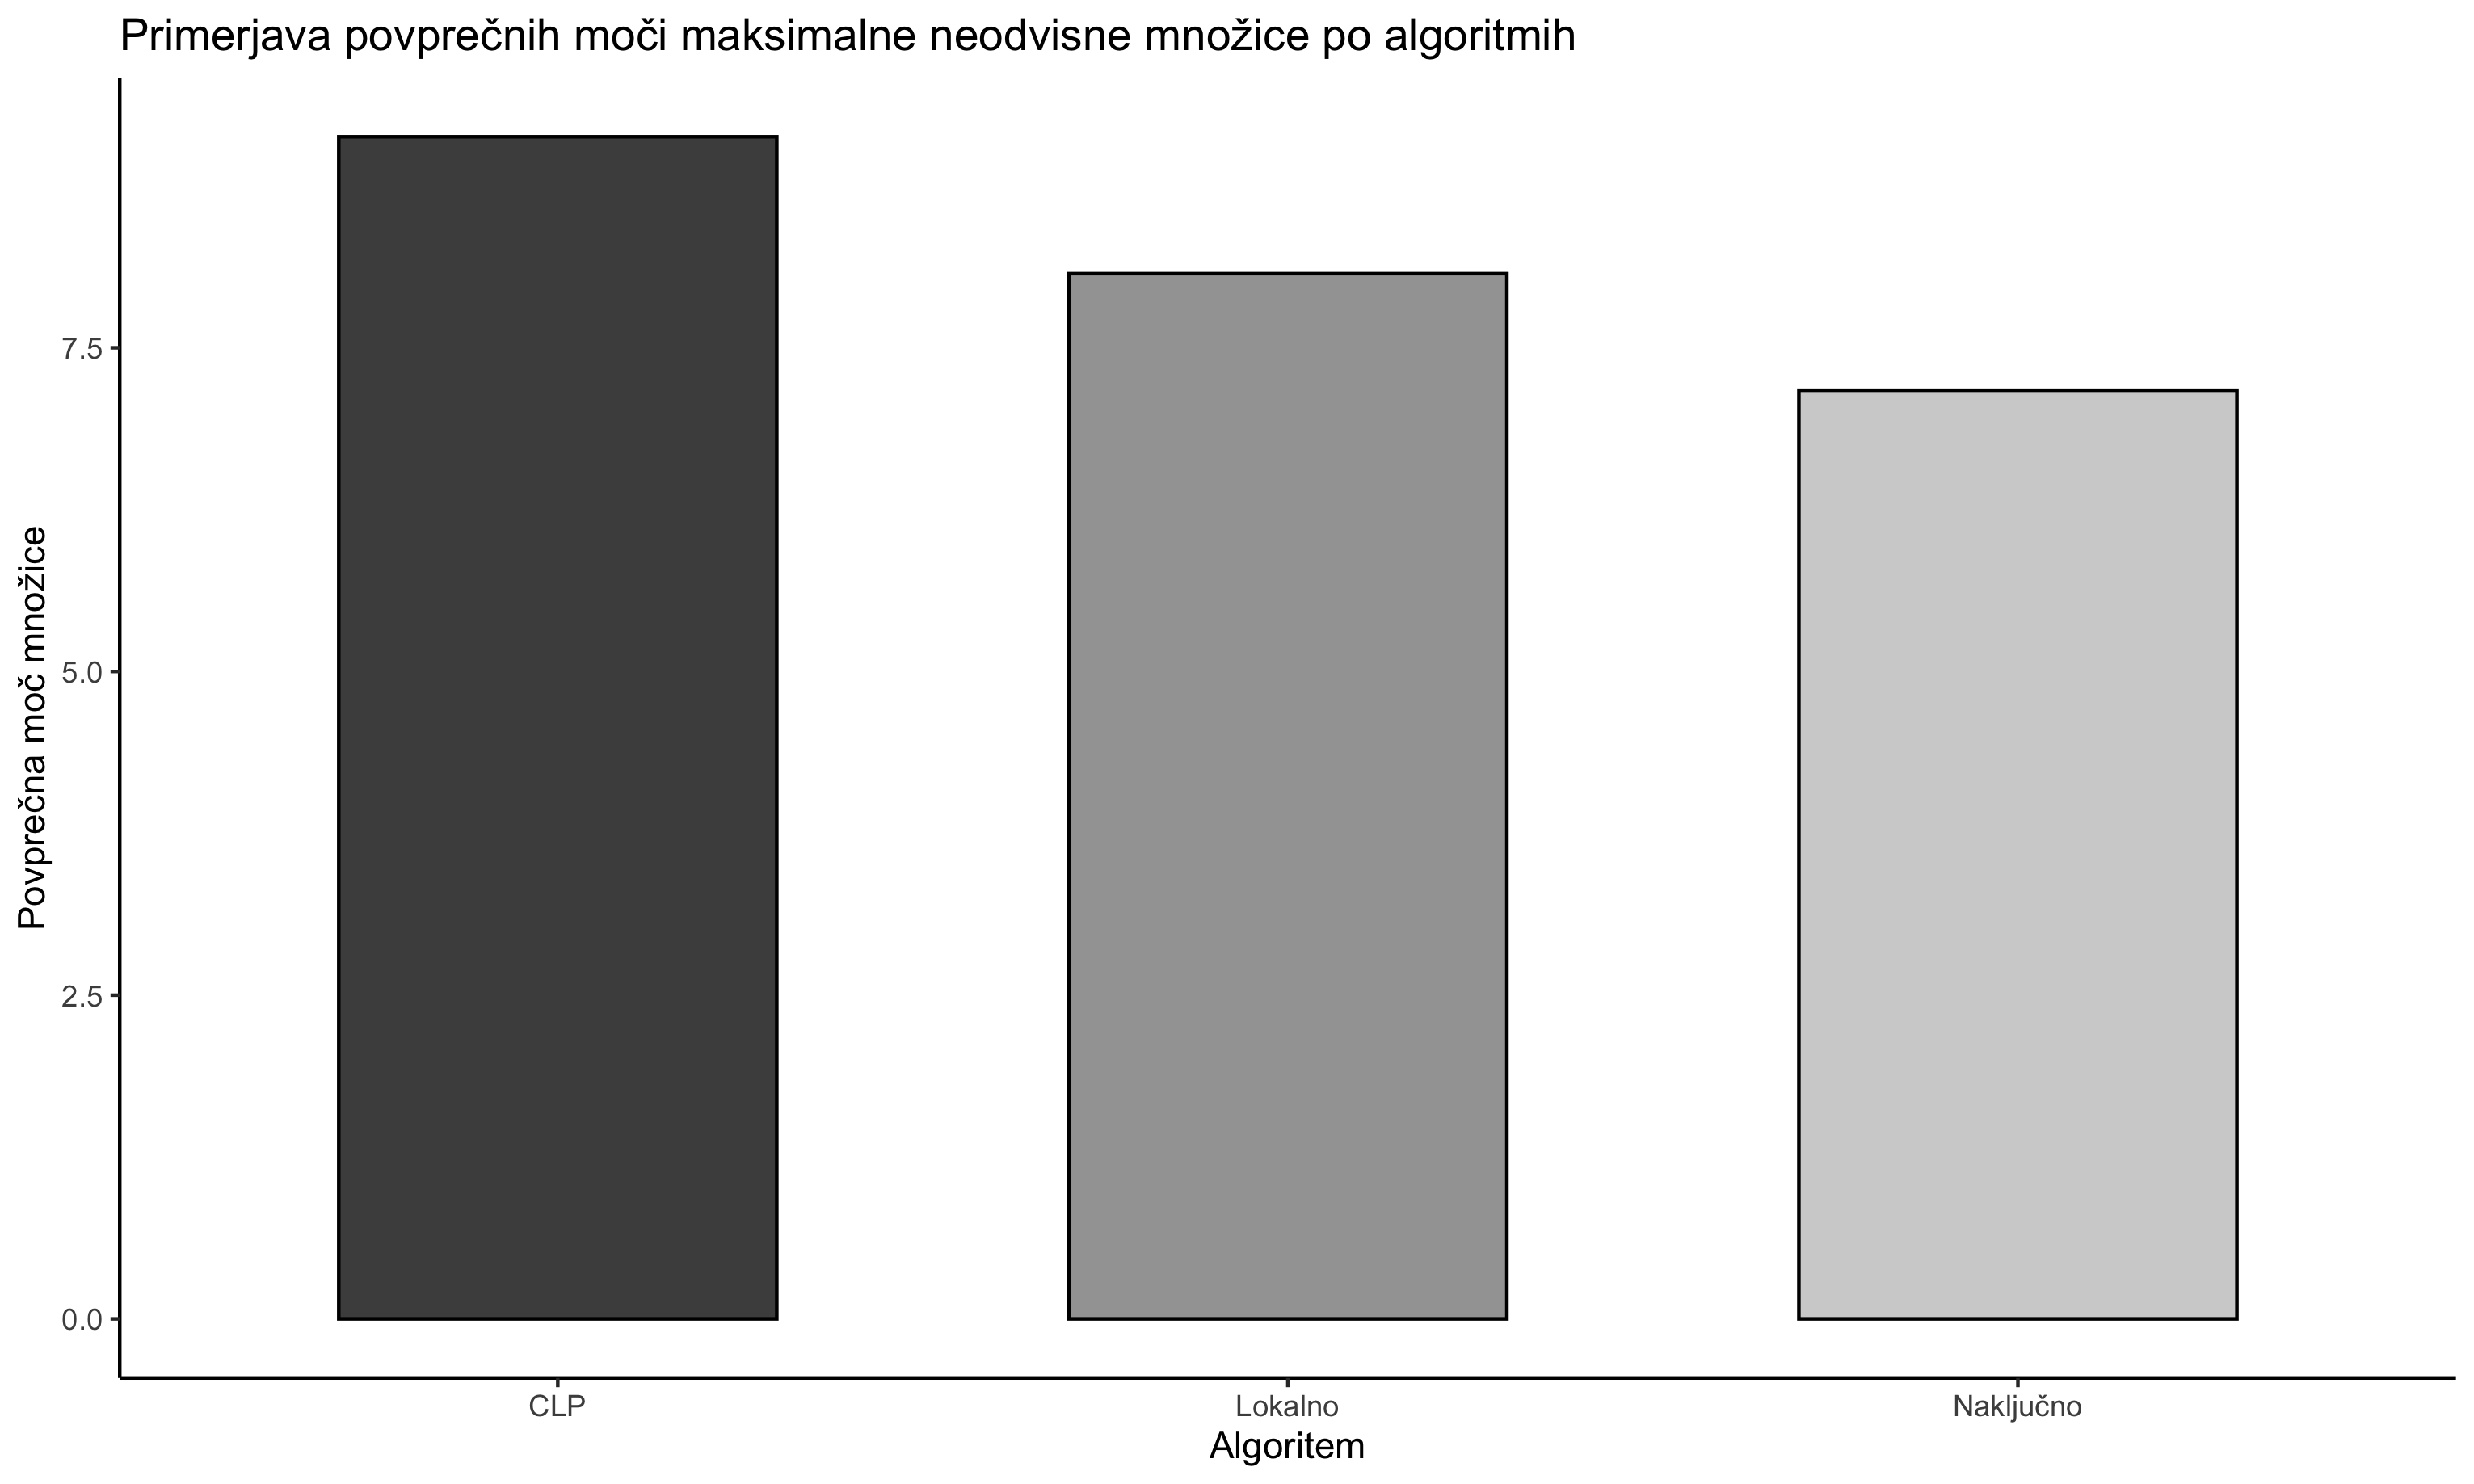
\includegraphics[width=\textwidth]{R_koda/pon-povpmoc.png}
		\caption{Časovnica SPACa.}
	\end{center}
\end{figure}
a
\begin{figure}[h!]
	\begin{center}
		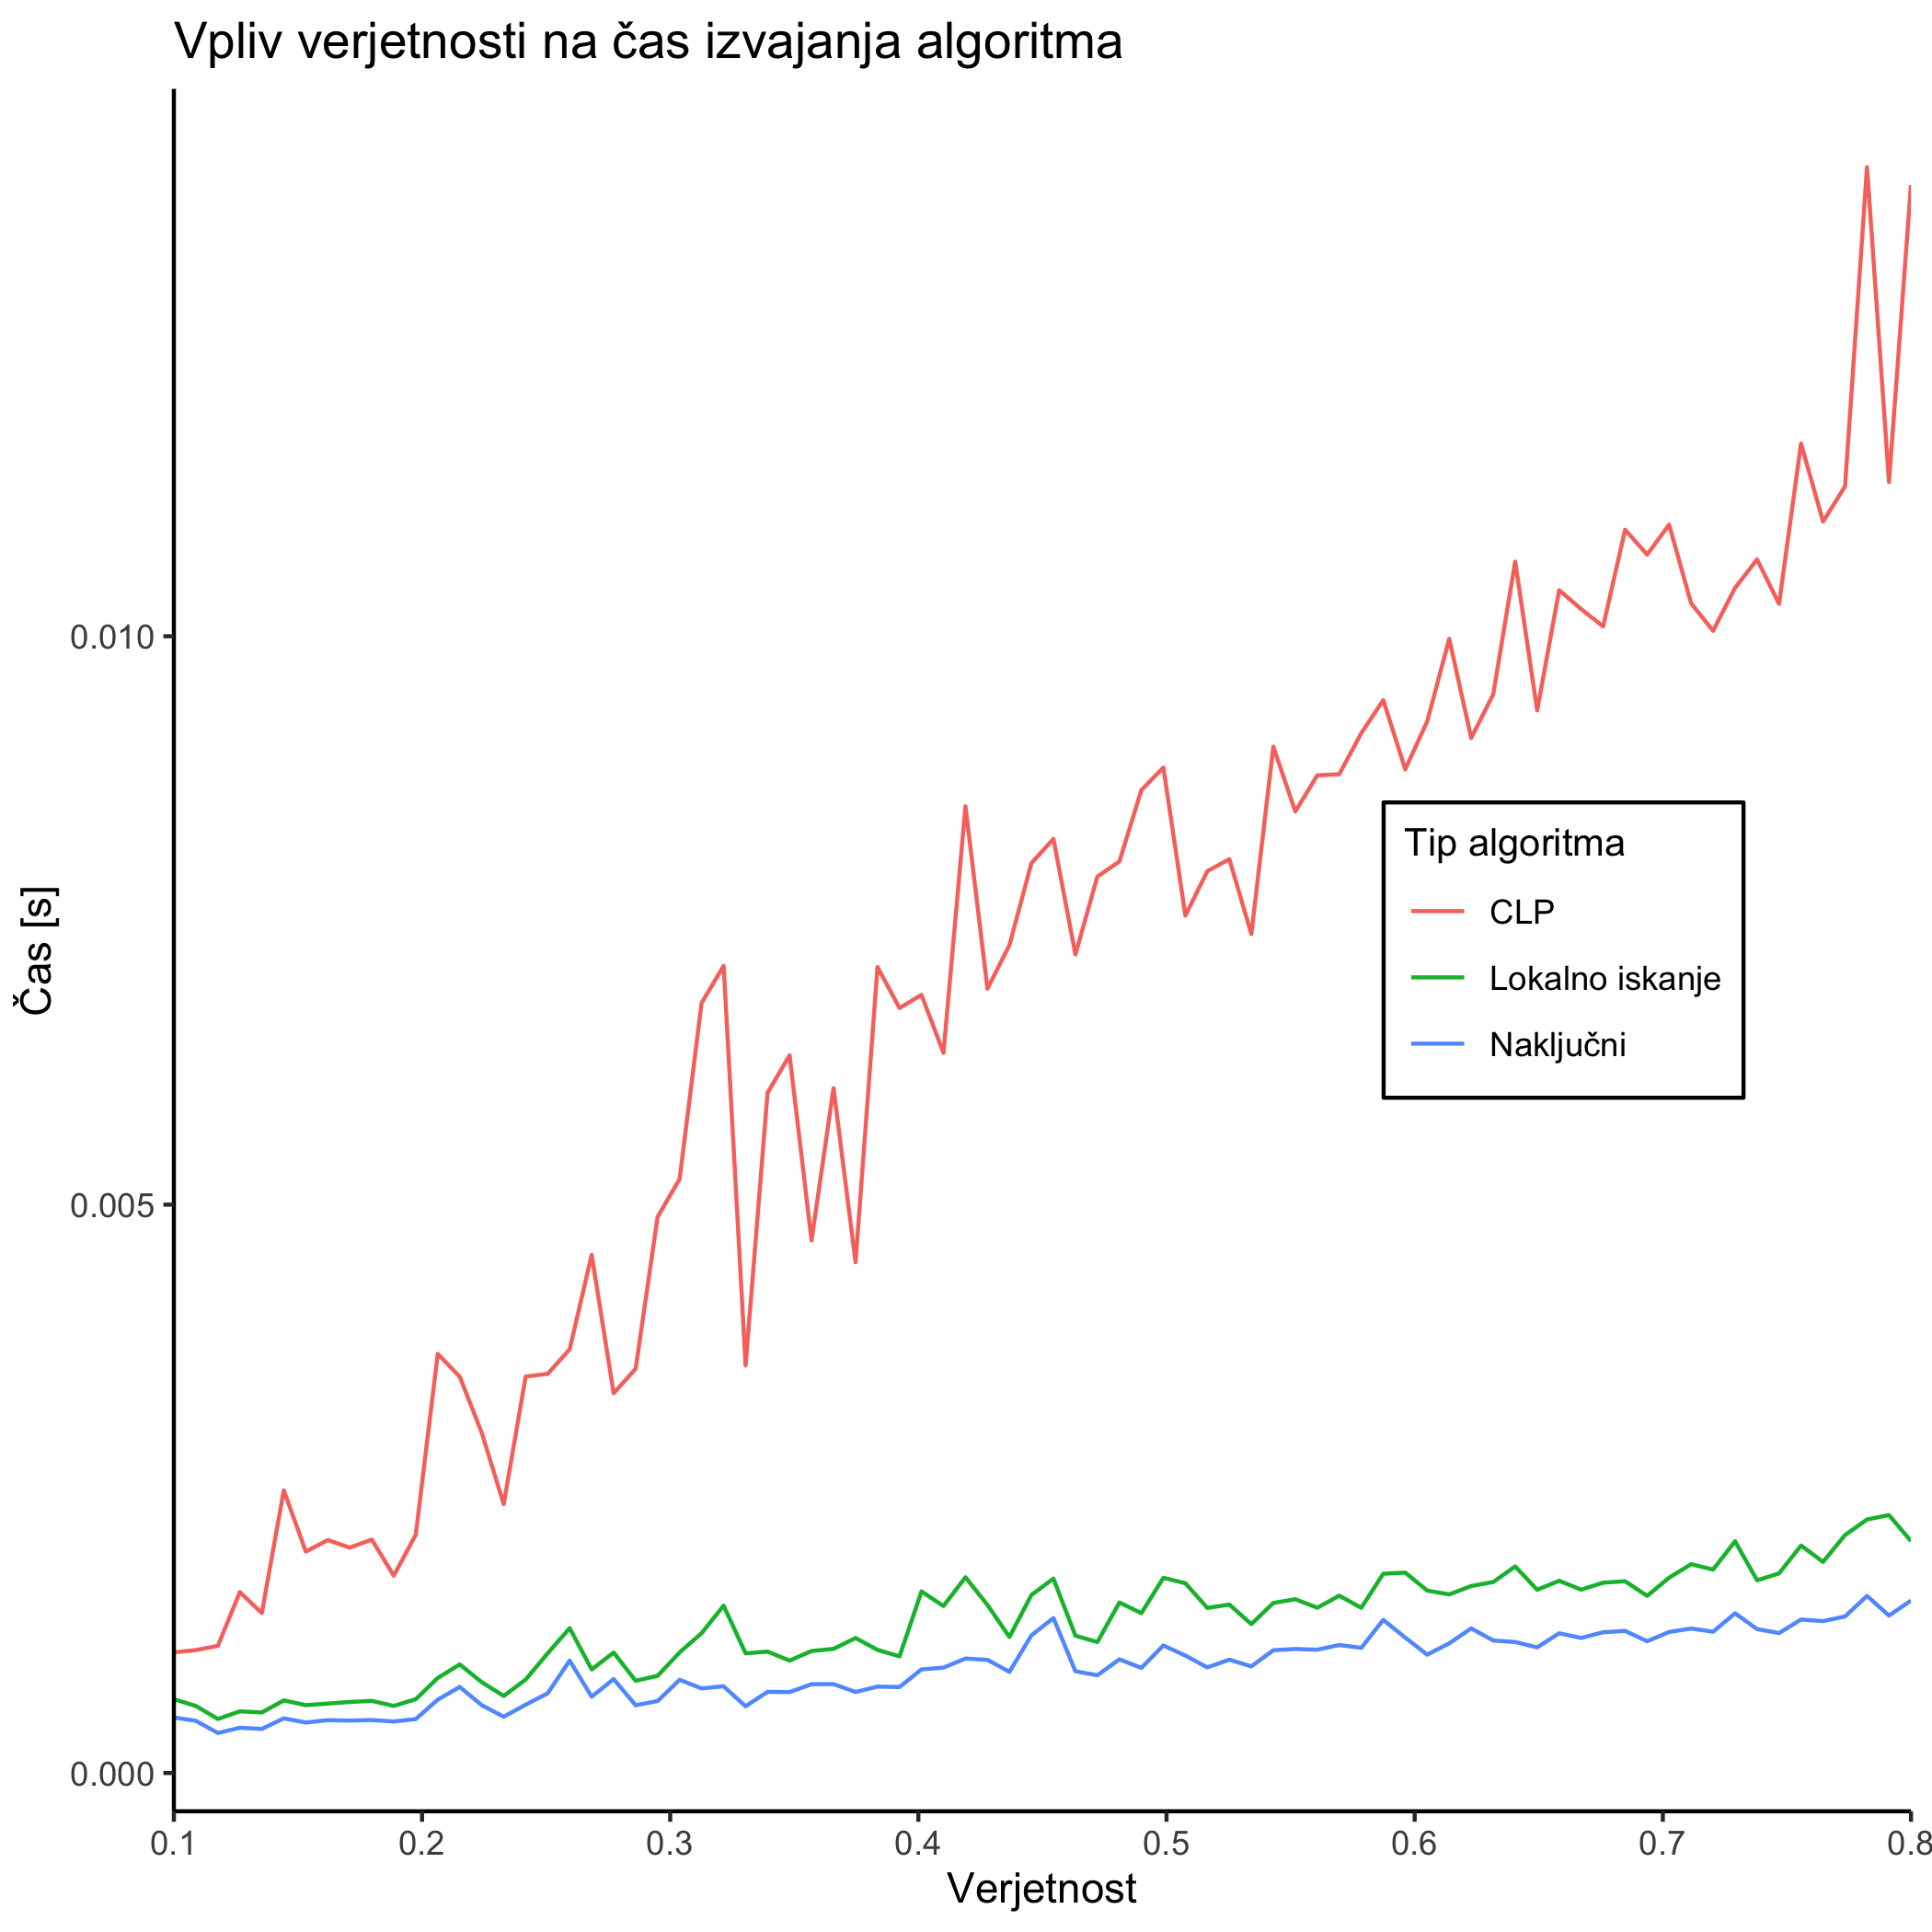
\includegraphics[width=\textwidth]{R_koda/ver-cas.png}
		\caption{Časovnica SPACa.}
	\end{center}
\end{figure}
a
\begin{figure}[h!]
	\begin{center}
		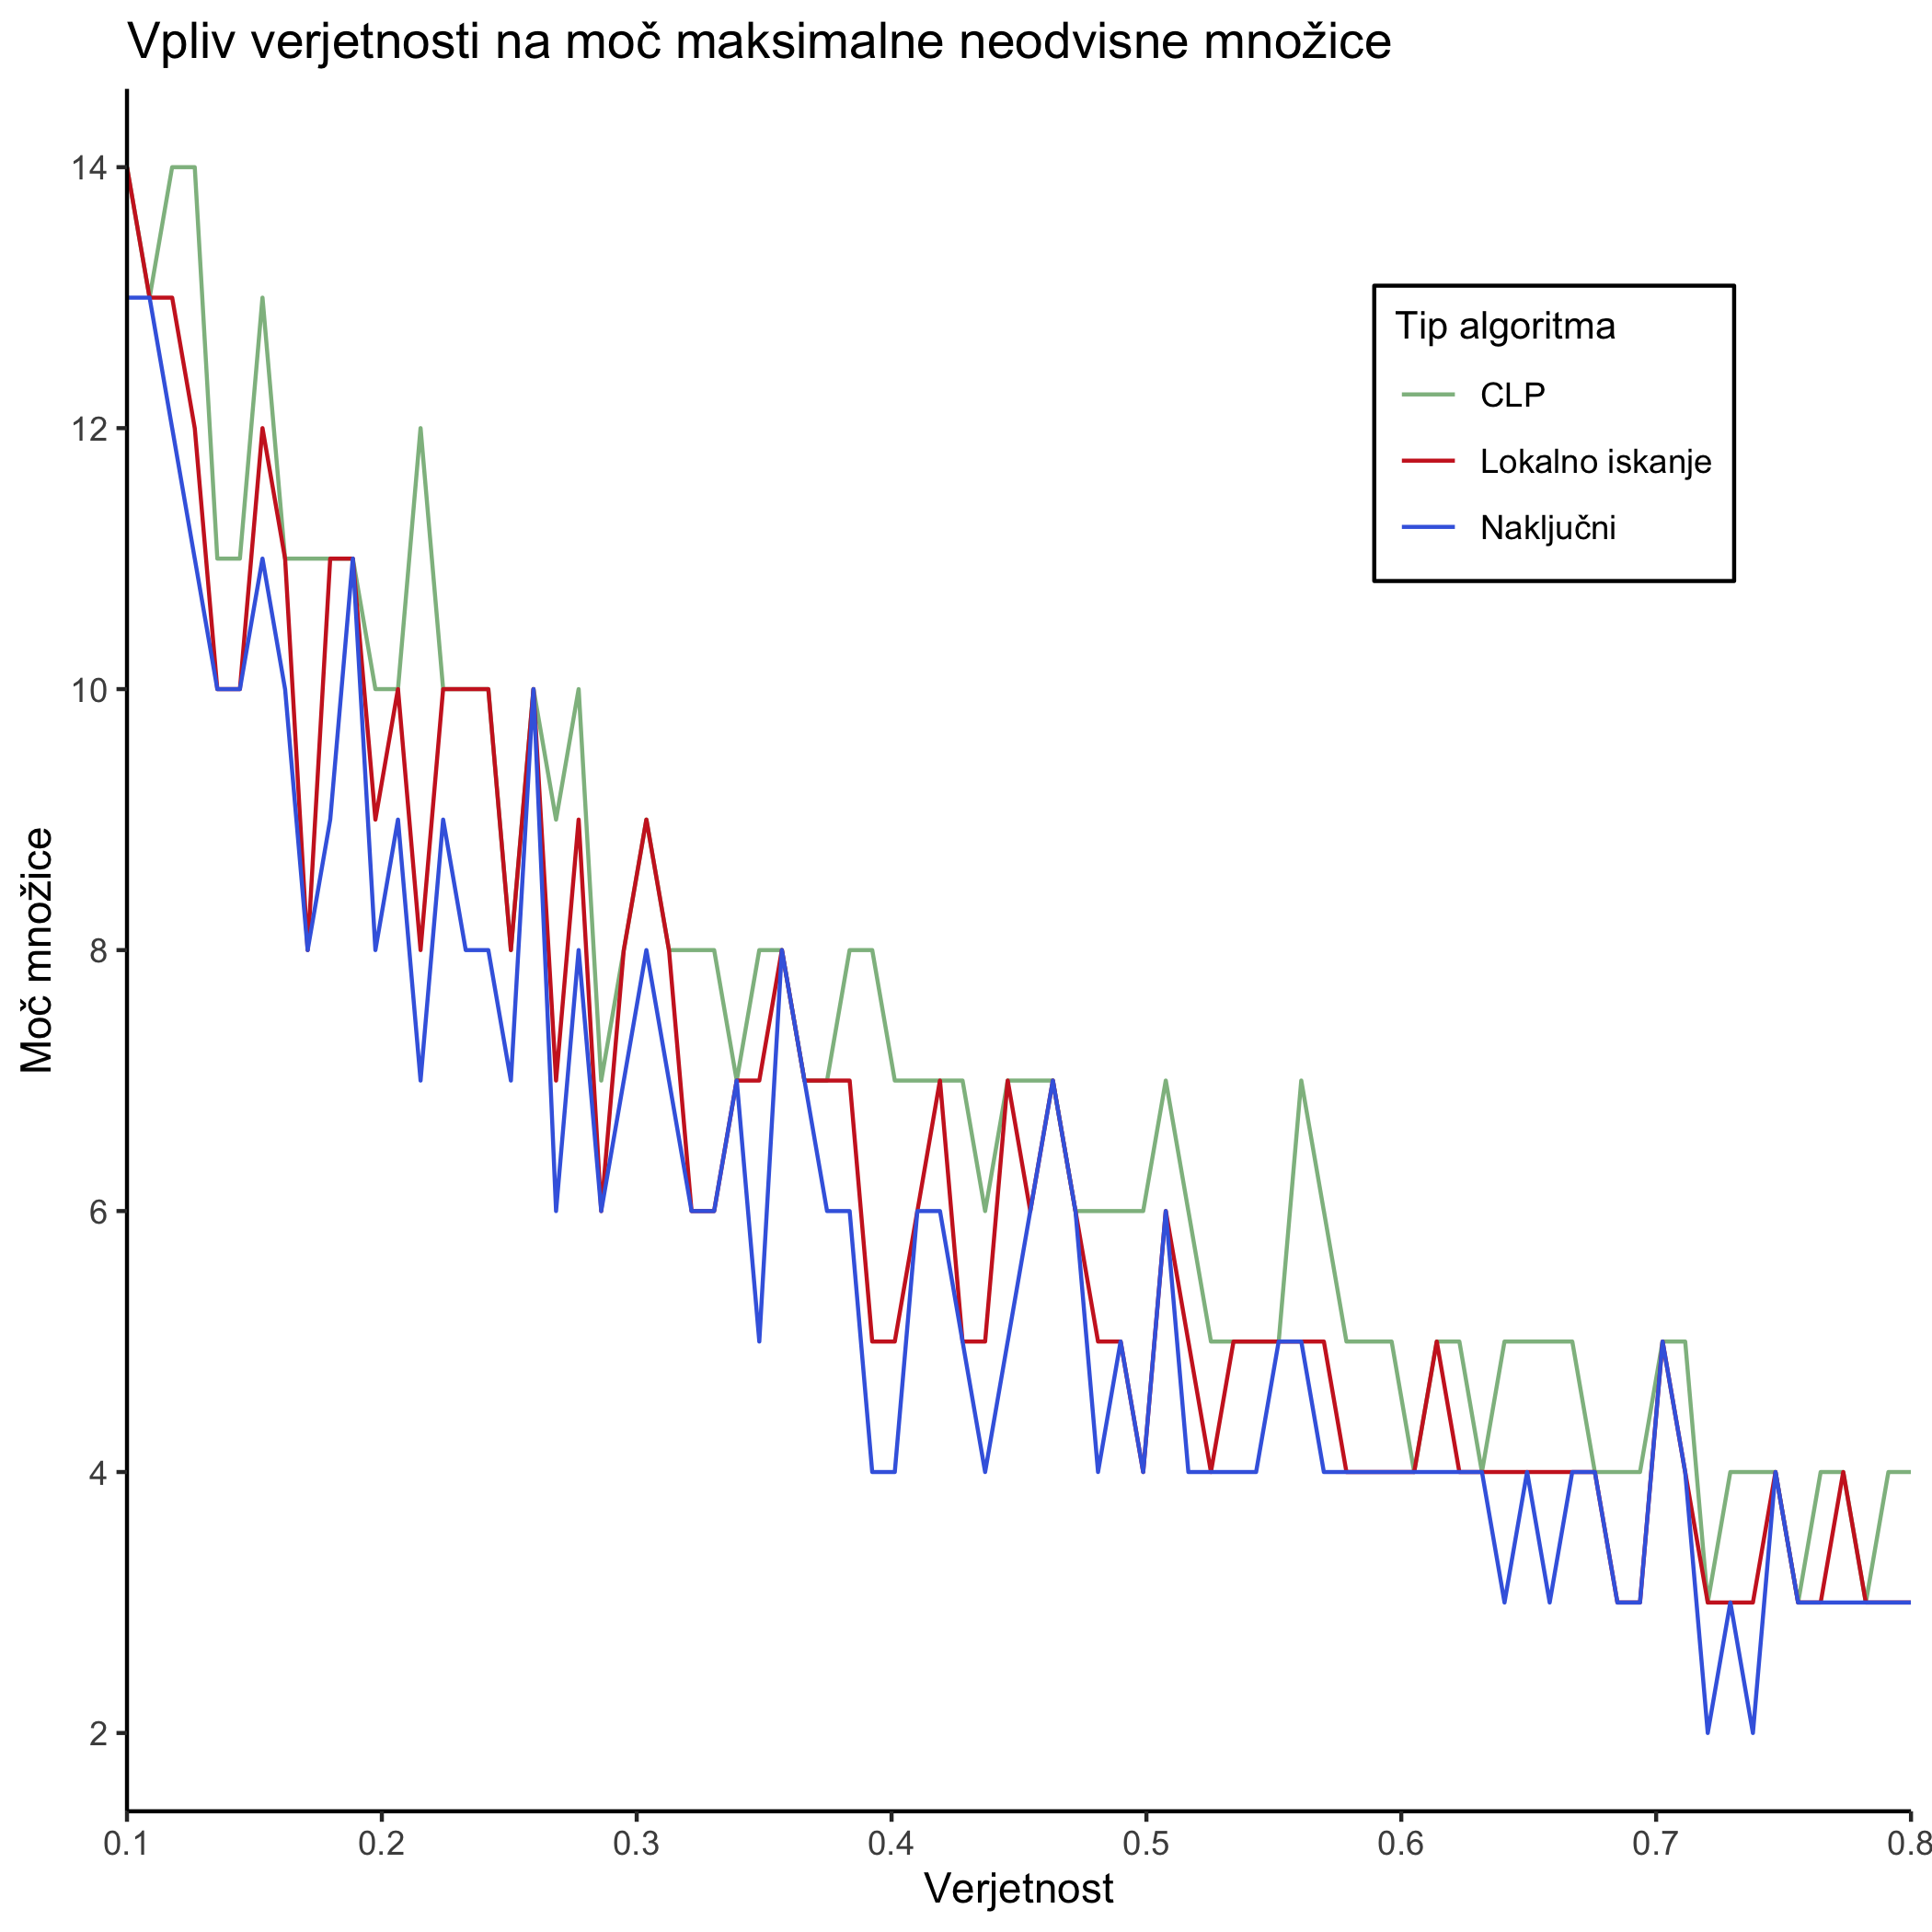
\includegraphics[width=\textwidth]{R_koda/ver-moc.png}
		\caption{Časovnica SPACa.}
	\end{center}
\end{figure}
a
\begin{figure}[h!]
	\begin{center}
		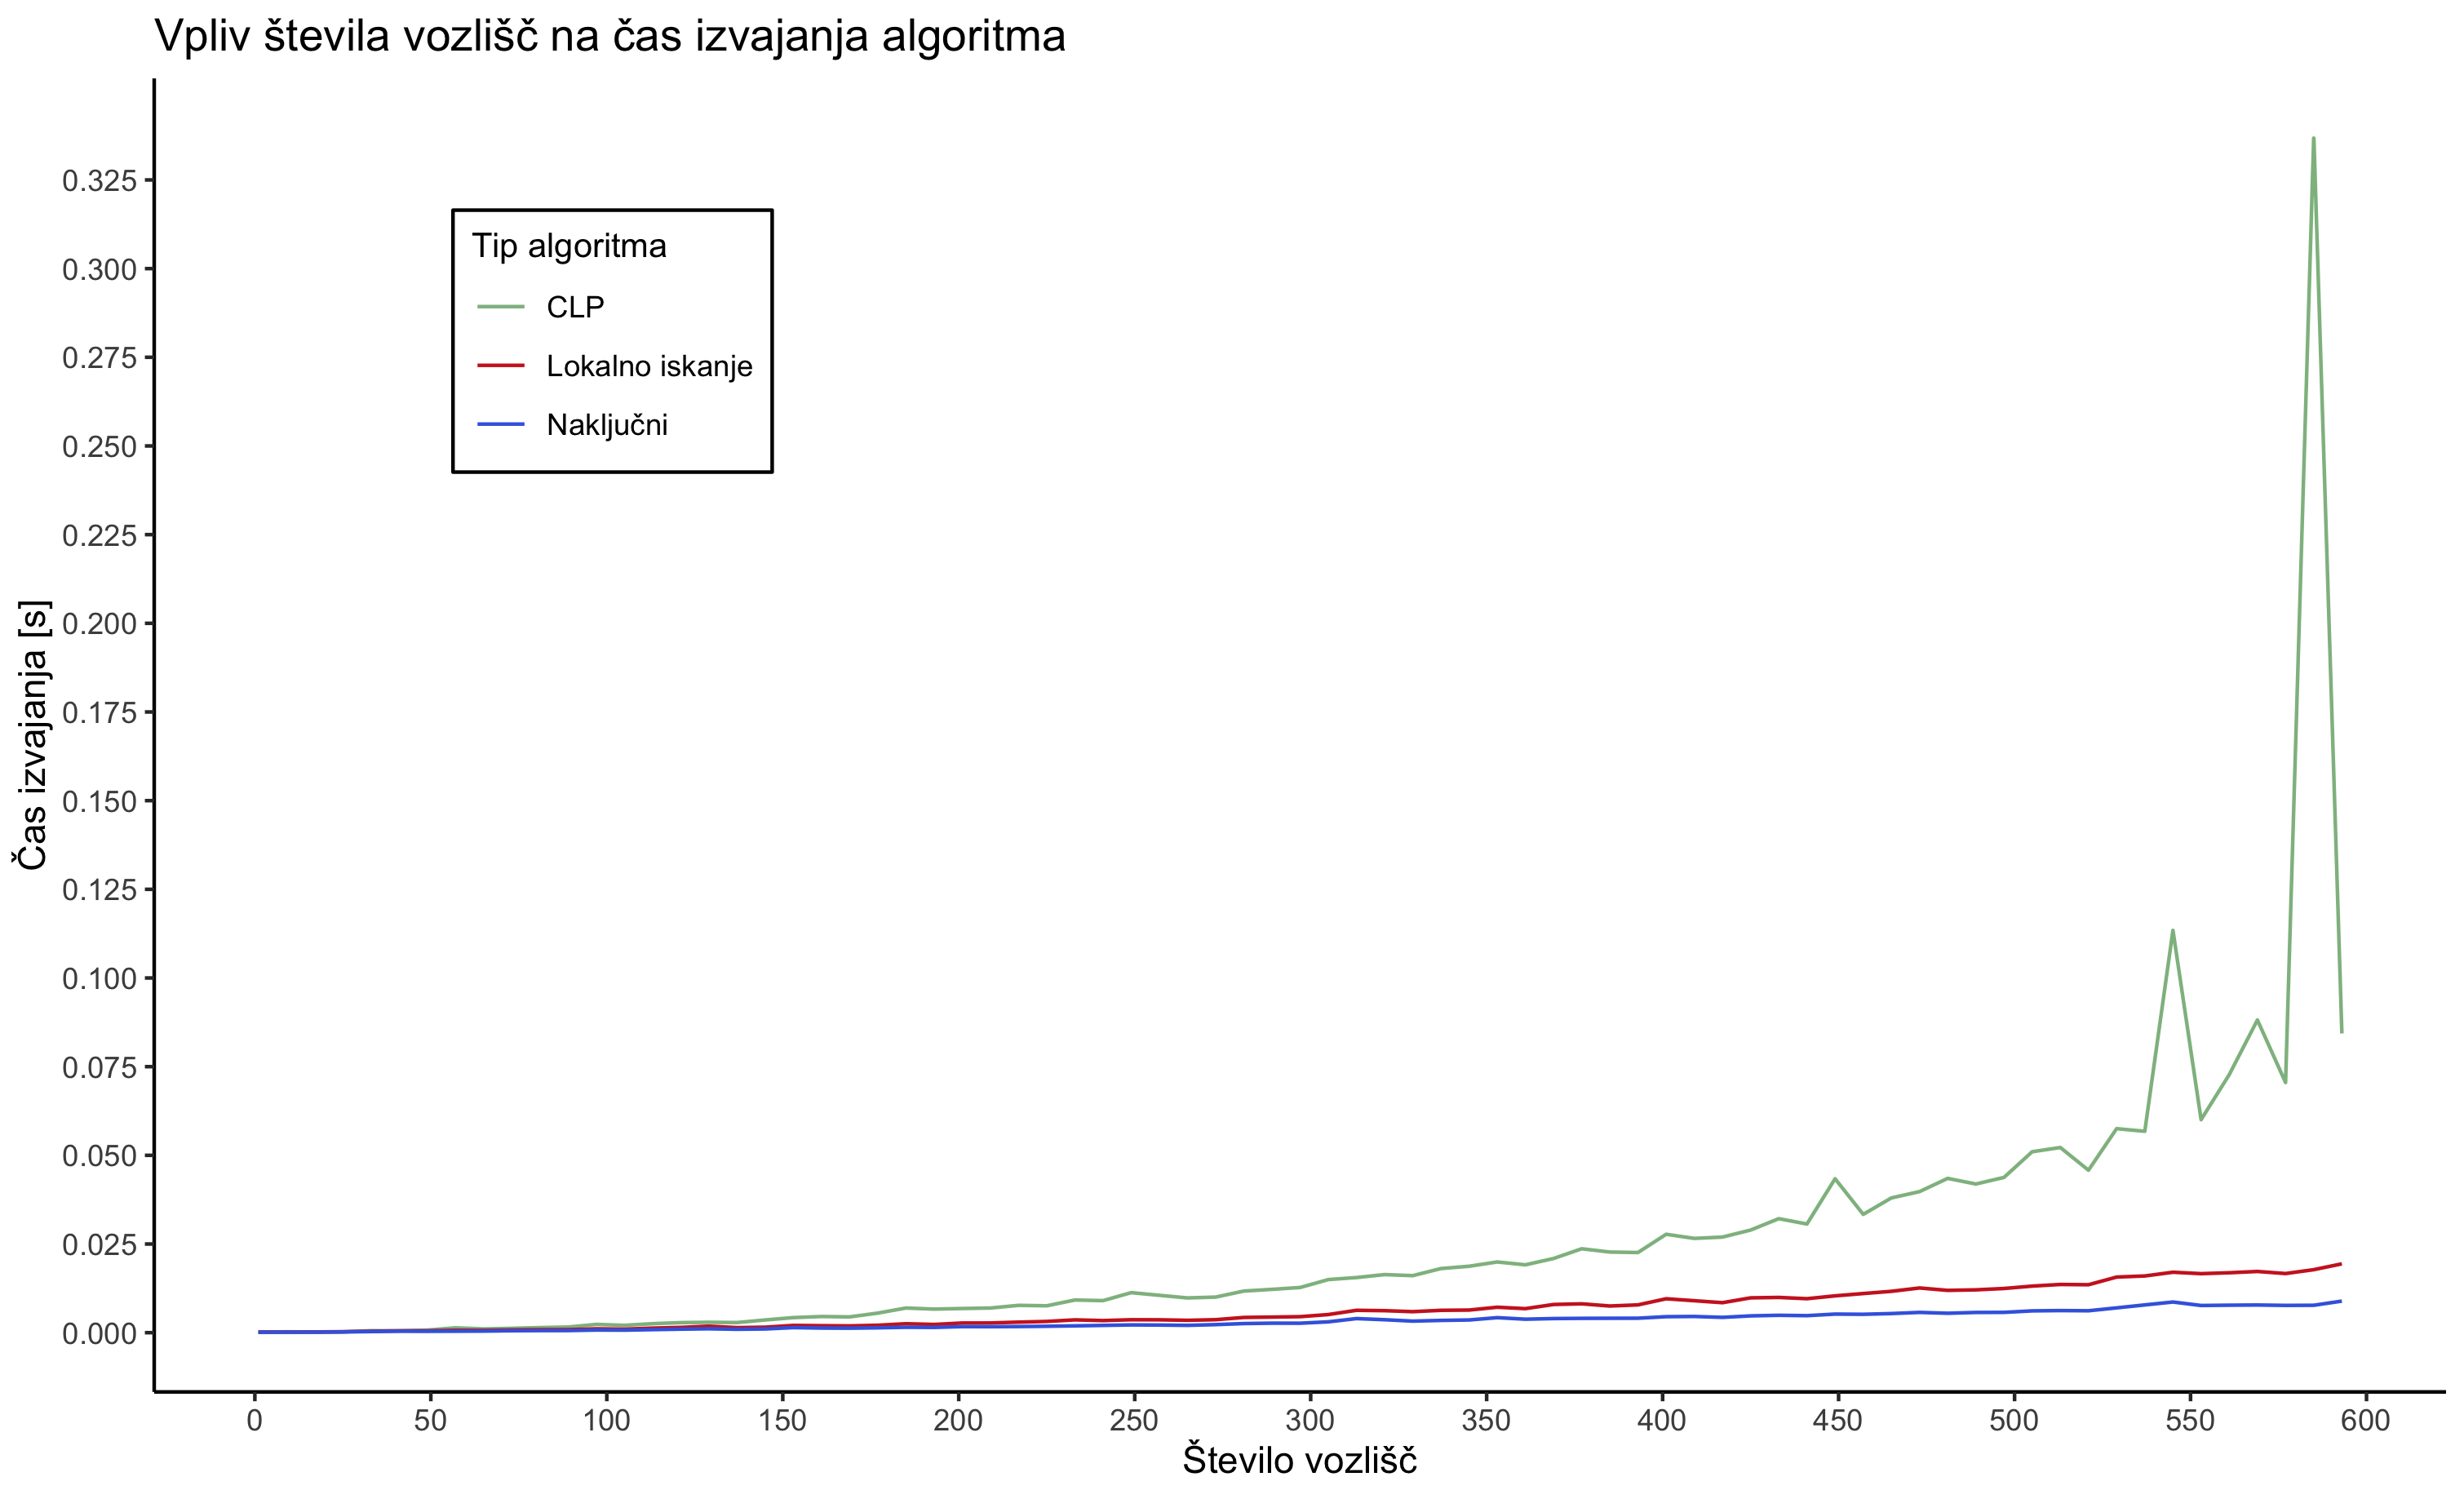
\includegraphics[width=\textwidth]{R_koda/voz-cas.png}
		\caption{Časovnica SPACa.}
	\end{center}
\end{figure}
a
\begin{figure}[h!]
	\begin{center}
		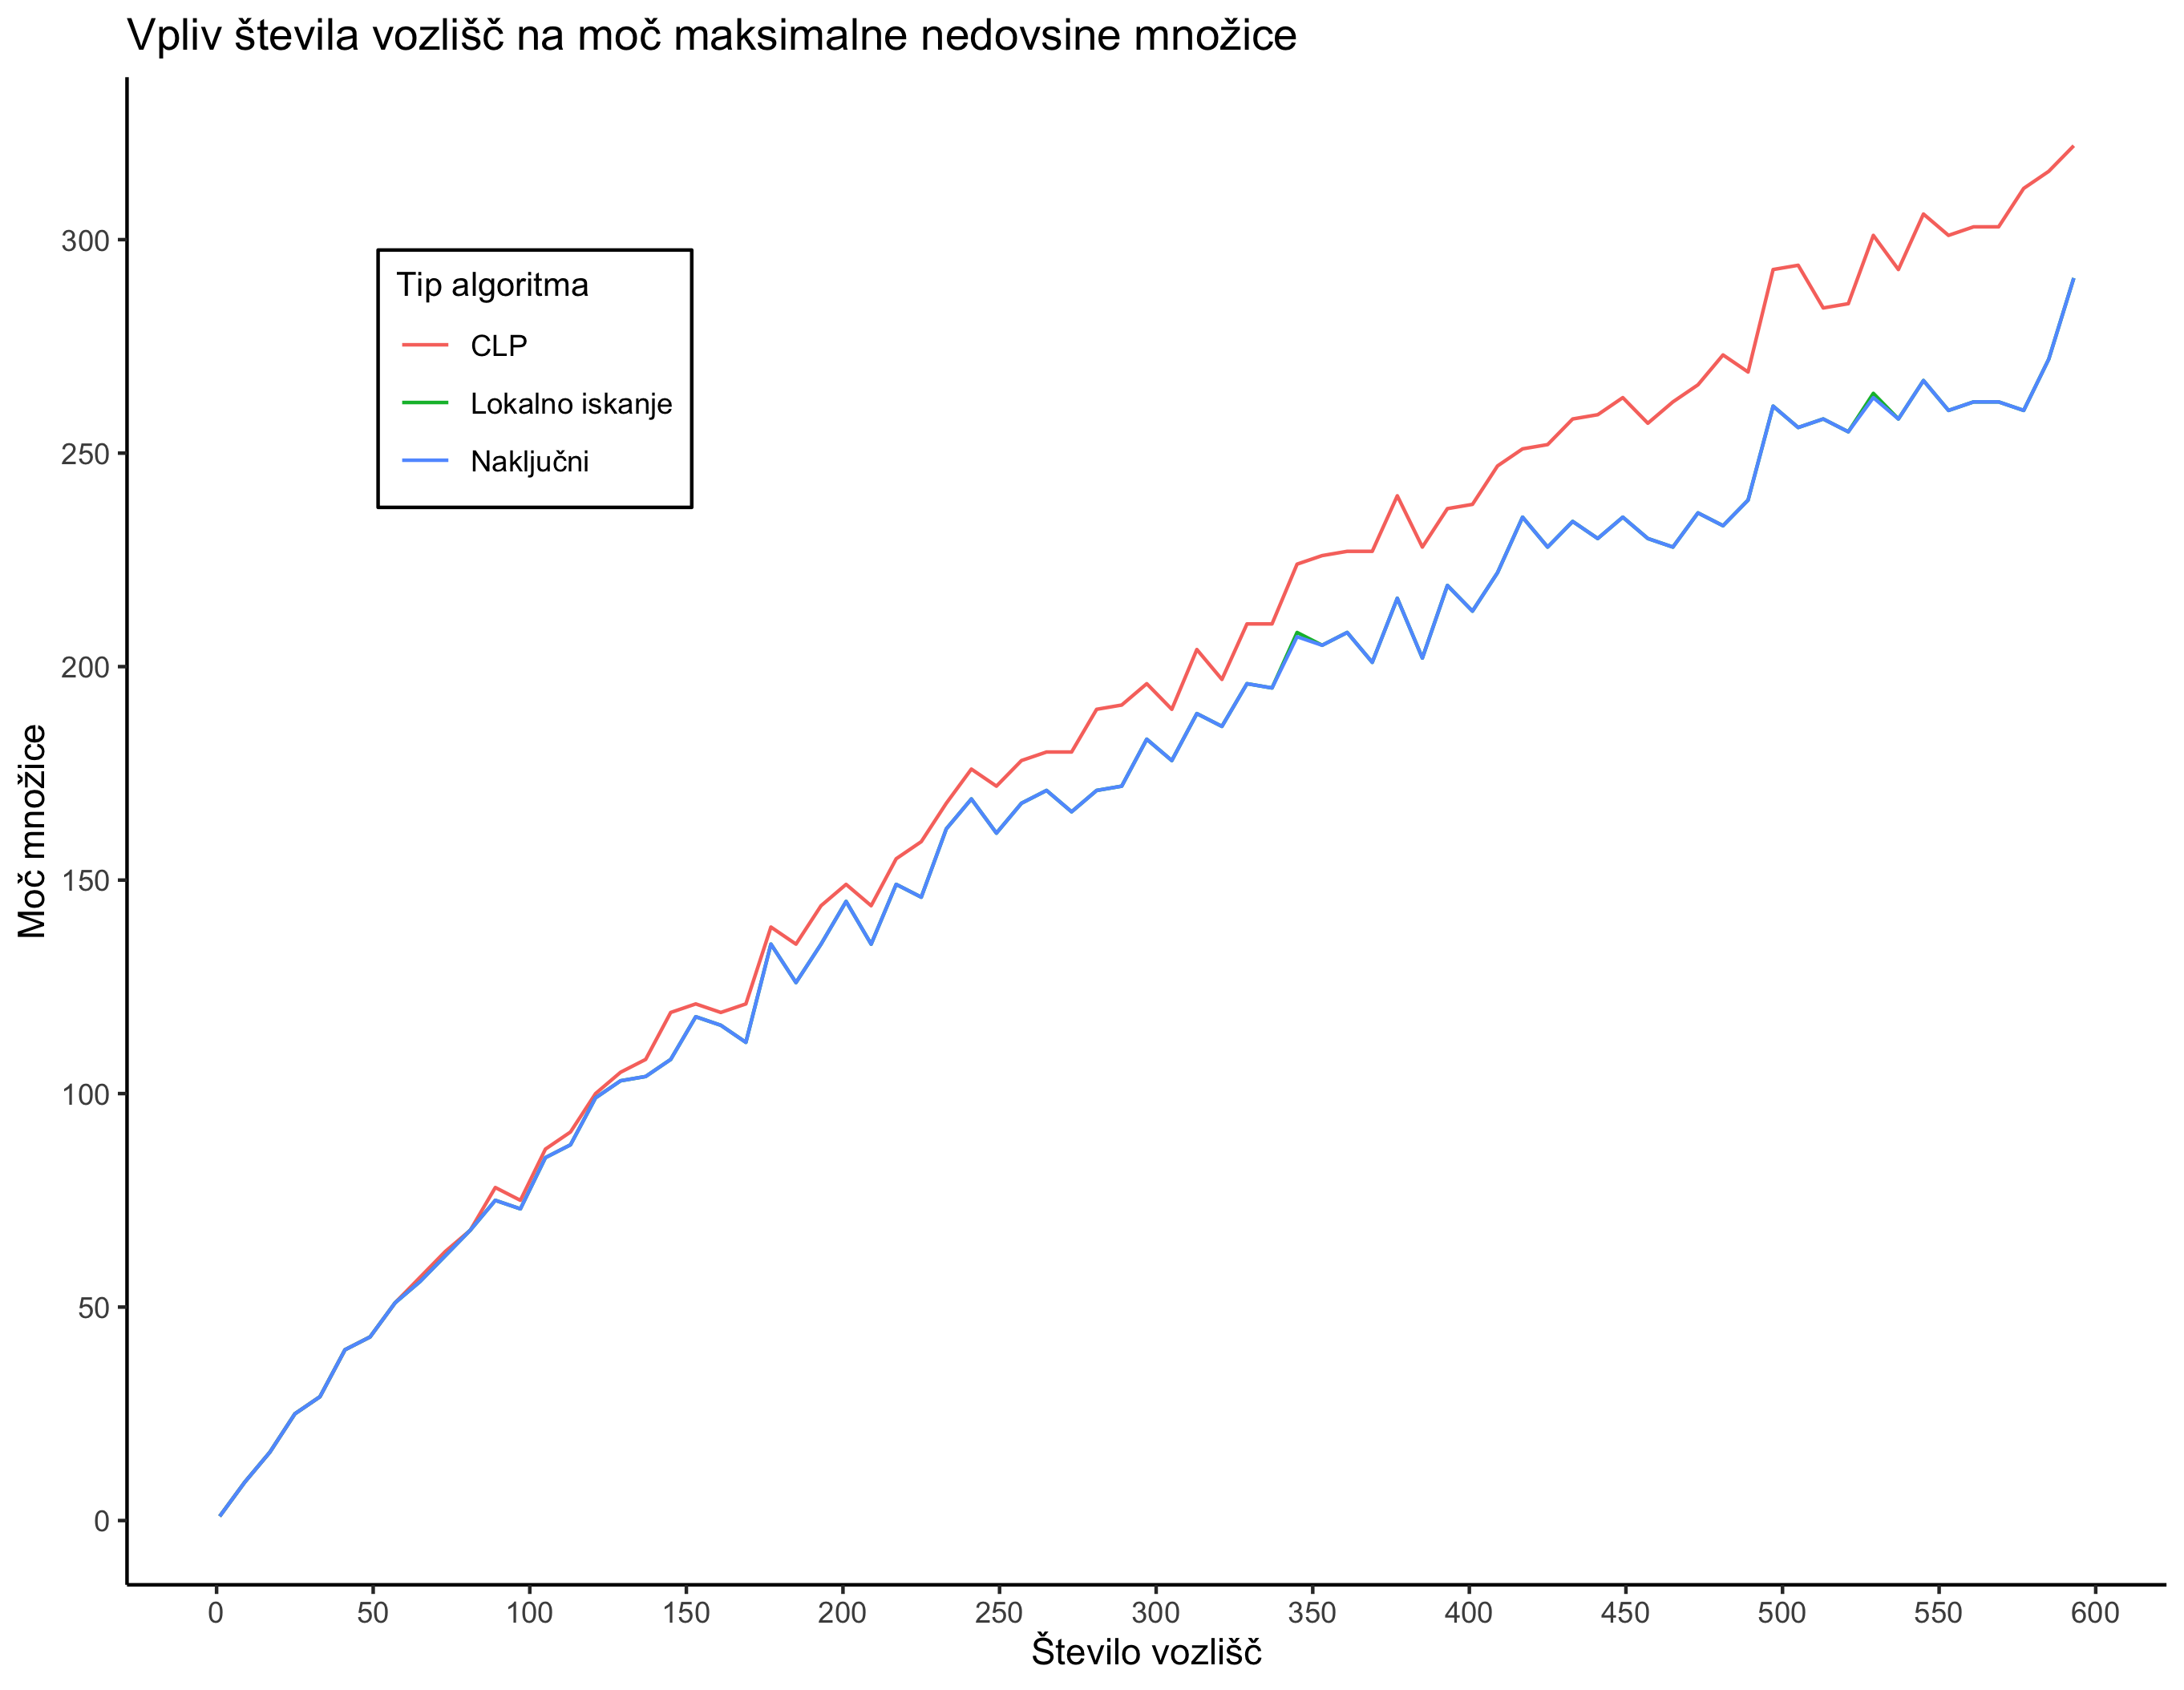
\includegraphics[width=\textwidth]{R_koda/voz-moc.png}
		\caption{Časovnica SPACa.}
	\end{center}
\end{figure}



\section{Sklep}

\newpage

\begin{thebibliography}{9}    

    \bibitem{Mil} 
    Gary Miller.
    \textit{Lecture 32: Luby’s Algorithm for Maximal Independent Set}, dostopno na \url{http://www.cs.cmu.edu/afs/cs/academic/class/15750-s18/ScribeNotes/lecture32.pdf}.
    \bibitem{And, Res} 

    Diogo Andrade, Mauricio G. C. Resende.
    \textit{Fast Local Search for the Maximum Independent Set Problem.} Conference Paper in Journal of Heuristics, May 2008, 
    dostopno na \url{https://www.researchgate.net/publication/221131653_Fast_Local_Search_for_the_Maximum_Independent_Set_Problem}.

    \bibitem{Wiki} 
    \textit{Maximal independent set}, v: Wikipedia: The Free Encyclopedia,[ogled 6.~1.~2022], dostopno na \url{https://en.wikipedia.org/wiki/Maximal_independent_set}.

    \bibitem{Wiki} 
    \textit{Independent set (graph theory)}, v: Wikipedia: The Free Encyclopedia,[ogled 6.~1.~2022], dostopno na \url{https://en.wikipedia.org/wiki/Independent_set_(graph_theory)}.

    
\end{thebibliography}

\end{document}